\documentclass[11pt,a4paper]{scrartcl}
%{{{ general stuff
\usepackage[english]{babel}
\usepackage[utf8]{inputenc}
\usepackage[T1]{fontenc}
\usepackage[hidelinks]{hyperref}
\usepackage{float} % use H in figure placement

%}}}
%{{{ graphics
\usepackage{graphicx} % Bilder
%}}}
%{{{ math
\usepackage{mathrsfs} % mathcal and mathscr
\usepackage{mathtools, amssymb, amsthm}
\usepackage{bm} % cool bold symbols
%}}}

% a todo command===============================================================
\newcounter{todocounter}
\newcommand{\todo}[2][noisnotdefined]{
 \marginpar{\fcolorbox{black}{yellow}{\footnotesize\textbf{todo}}
 \ifthenelse{\equal{#1}{noisnotdefined}}{}{\textcolor{black}{\newline\tiny #1}}}
 \textbf{\ifthenelse{\equal{#2}{.}}
   {\fcolorbox{blue}{white}{\textcolor{blue}{$\maltese$}}}{{\textcolor{blue}{#2}}}}
 \refstepcounter{todocounter}}

%===============================================================================

\date{}

\begin{document}

\section*{Project Proposal for Genetic Algorithms and Evolutionary Programming
by Felix Bartel and D\` avid Kerekes}

Our idea was to apply a genetic algorithm to a neuronal network which is known as neuroevolution.
A big advantage of this sheme is that one only needs an indicator how good the neuronal network is given a certain task.
This can for instance be given by the outcome of a game.
Our game of choice was Blobby Volly 2 which is a simple two-dimensional vollyball game with open source written in C++ with lua support, cf. Figure \ref{fig:screenshot}.

\begin{figure}[H]
\center
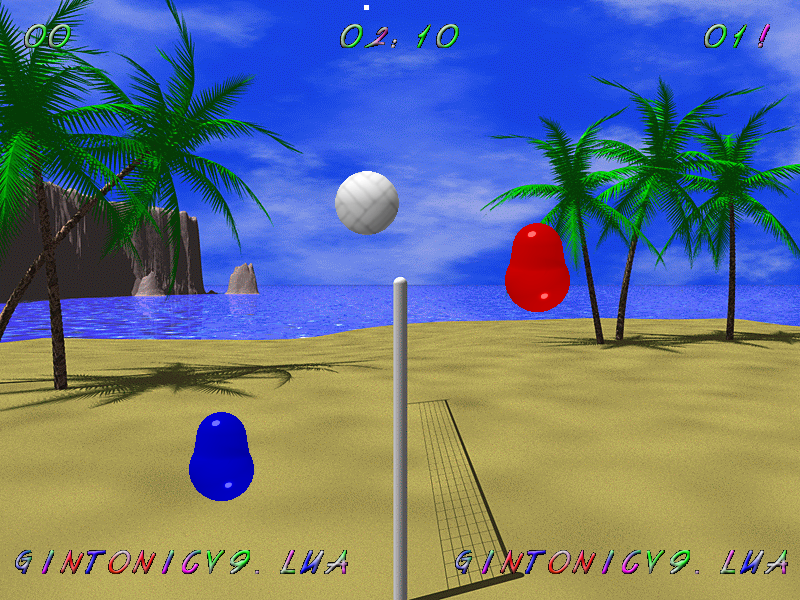
\includegraphics[width=0.7\textwidth]{img/screenshot.png}
\caption{screenshot of the game}
\label{fig:screenshot}
\end{figure}

A scene from the game could be described by the $x$ and $y$ coordinates of the players and the ball, their corresponding velocities and the current number of ball contacts.
These arguments or a subset of them could then be used as input for the neuronal network.
The output would then be the players movement which only consists of going right, left or jumping.
Assuming the layers of the neuronal network have $n_1,\dots,n_L$ nodes we then have to optimize a function of $\sum_{l=1}^{L-1} n_ln_{l+1}$ variables if we fix the size of the network.
A few possible extensions are
\begin{itemize}
\item different crossover operators
\item differnet mutation operators (maybe use a covanriance matrix, if the size allows it)
\item make the size of the network variable
\item vary the input or output nodes
\item vary the opponent to train (maybe also the neuronal network itself)
\end{itemize}


\end{document}
